%% Template for a preprint Letter or Article for submission
%% to the journal Nature.
%% Written by Peter Czoschke, 26 February 2004
%%

\documentclass{nature}
%\documentclass[12pt]{article}

%% make sure you have the nature.cls and naturemag.bst files where
%% LaTeX can find them

\bibliographystyle{naturemag}

\usepackage{graphicx}
\usepackage{amssymb,amsfonts,amsmath}
\usepackage{subfigure}
\usepackage{stfloats}


%% OPTIONAL MACRO DEFINITIONS
\def\s{\sigma}
\newcommand{\be}[0]{\begin{equation}}
\newcommand{\ee}[0]{\end{equation}}
\newcommand{\lb}[0]{\left(}
\newcommand{\rb}[0]{\right)}
\renewcommand{\figurename}{Supplementary Figure}

%\title{Inefficacy of stratospheric sulfate aerosol injections for saving the West Antarctic Ice Sheet} % 94chars
%\title{Inefficacy of geoengineering by stratospheric aerosols for saving the West Antarctic Ice Sheet} 
%\title{Geoengineering by stratospheric sulfate aerosols cannot save the West Antarctic Ice Sheet} % 89
\title{Stratospheric sulfate aerosol injections cannot preserve the West Antarctic Ice Sheet} % 81
%\title{Ineffective preservation of the West Antarctic Ice Sheet under stratospheric sulfate aerosol injections}

%% Notice placement of commas and superscripts and use of &
%% in the author list


\author{K. E. McCusker*,$^{1,2}$ \& D. S. Battisti,$^{2}$ \& C. M. Bitz$^2$}

% NatGeo requirements:
% Title If possible, the title should give a sense of the main new finding, and should not exceed 90 characters, including spaces. Nature Geoscience titles do not contain technical terms or abbreviations unless absolutely necessary. We strongly discourage punctuation or active verbs.@@
% Letter 2,000 words no methods, 3 figures
% Article 3,000 words no methods, include section titles, 6 figures. No refs in abstract. ~500 words of Intro. 1-2 para of conclusions


\begin{document}

\maketitle

\begin{affiliations}
 \item Department of Atmospheric Sciences, University of Washington, Seattle, WA 98195, USA
 \item School of Earth and Ocean Sciences, University of Victoria, Victoria, BC, V8V 1B5, Canada
\end{affiliations}

\section*{Supplementary Figures}

%%%%%%% supplementary %%%%%%%

\begin{figure*}[Supplementary Figure]%[htbp] % the star afterwards makes it a one column fig in a 2-col document
%\centering
\noindent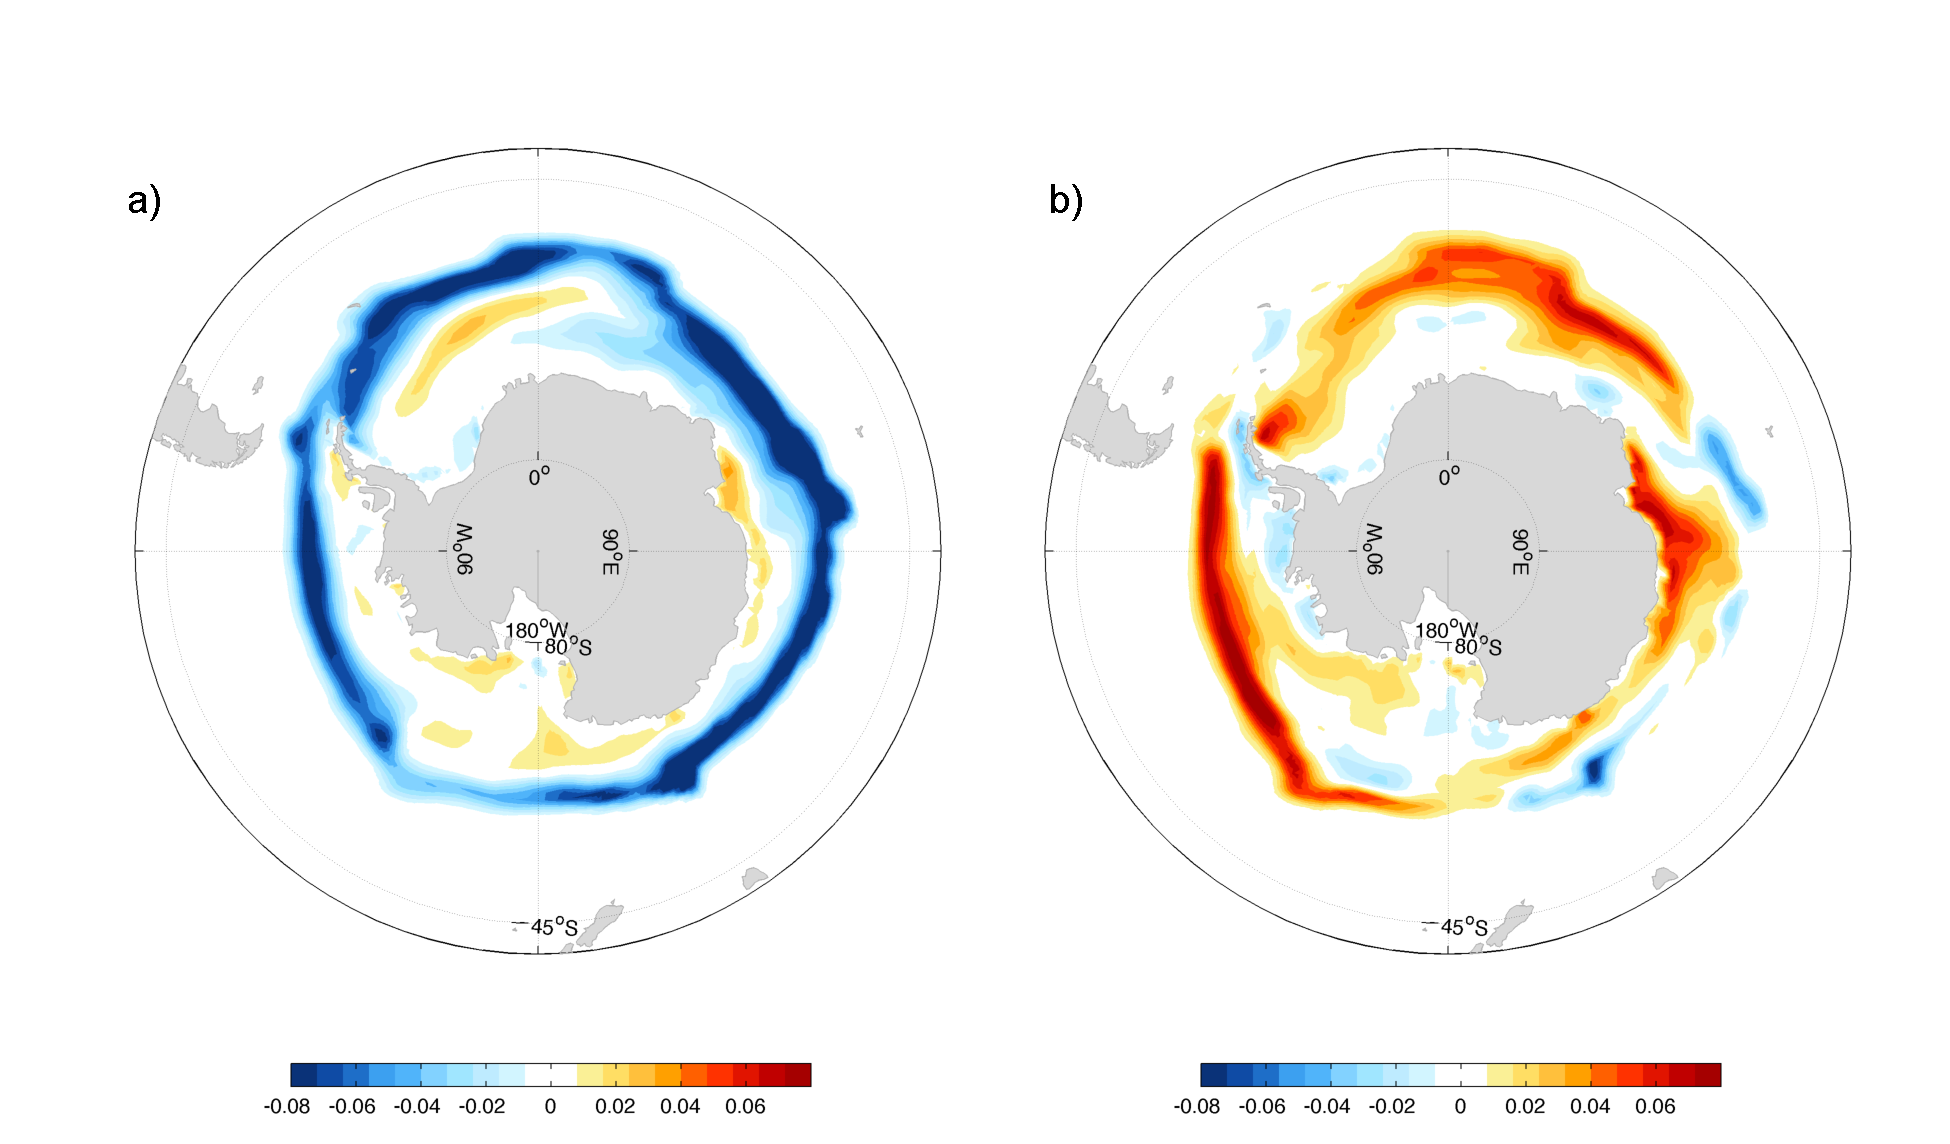
\includegraphics[width=39pc]{figures/SuppFig1.pdf}  % @@  reconfigure to horizontal layout?
\caption{\textbf{Sea ice concentration anomaly maps.} Annual average sea ice concentration (fraction) anomaly from 20thC (1970-1999 mean) for \textbf{(a)} Sulf and \textbf{(b)} GHGrem, years 2045-2054.}
\label{fig:supp1}
\end{figure*}

\begin{figure*}%[htbp] % the star afterwards makes it a one column fig in a 2-col document
%\centering
\noindent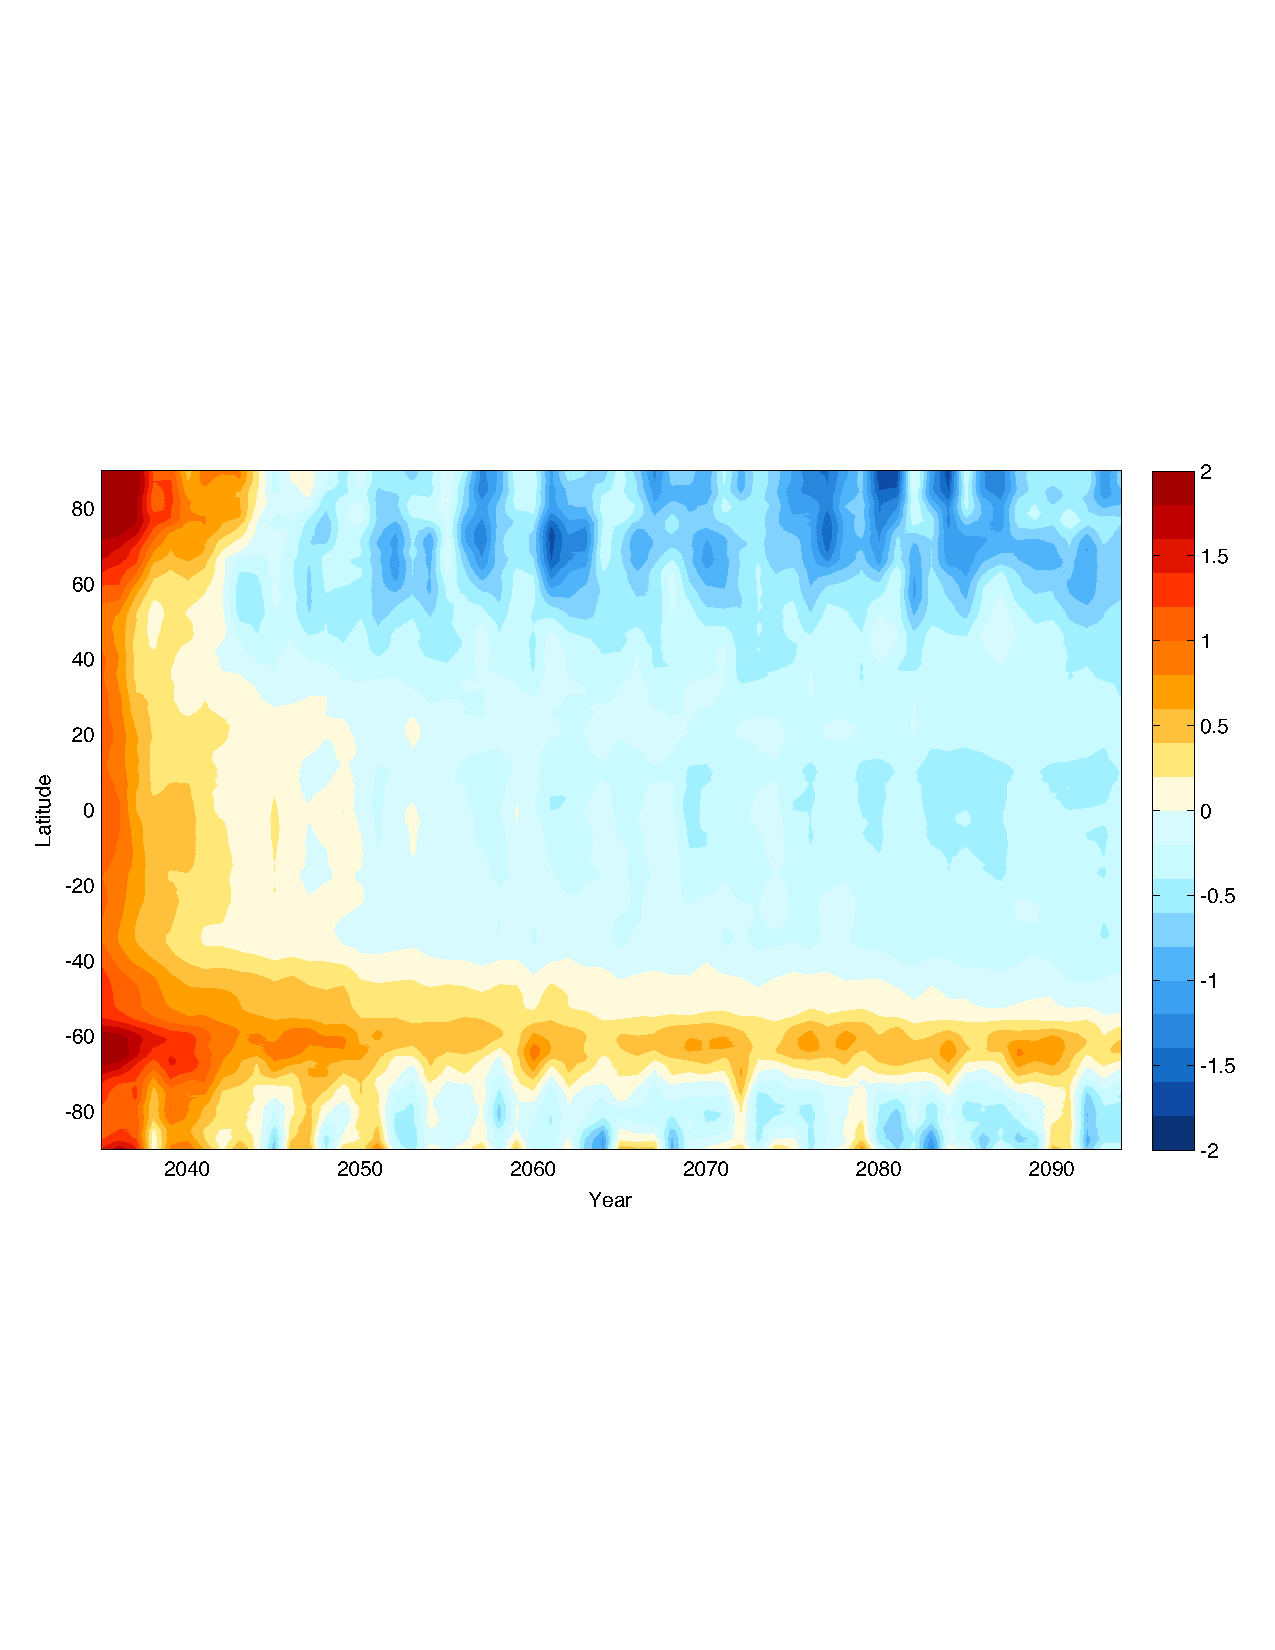
\includegraphics[width=39pc]{figures/SuppFig2.pdf}  % @@  reconfigure to horizontal layout?
\caption{\textbf{Zonal average SAT anomalies with time.} Annual average, zonal average Sulf surface air temperature ($^\circ$C) with latitude and time as anomalies from the 1970-1999 average from 20thC.}
\label{fig:supp2}
\end{figure*}

\begin{figure*}%[htbp] % the star afterwards makes it a one column fig in a 2-col document
%\centering
\noindent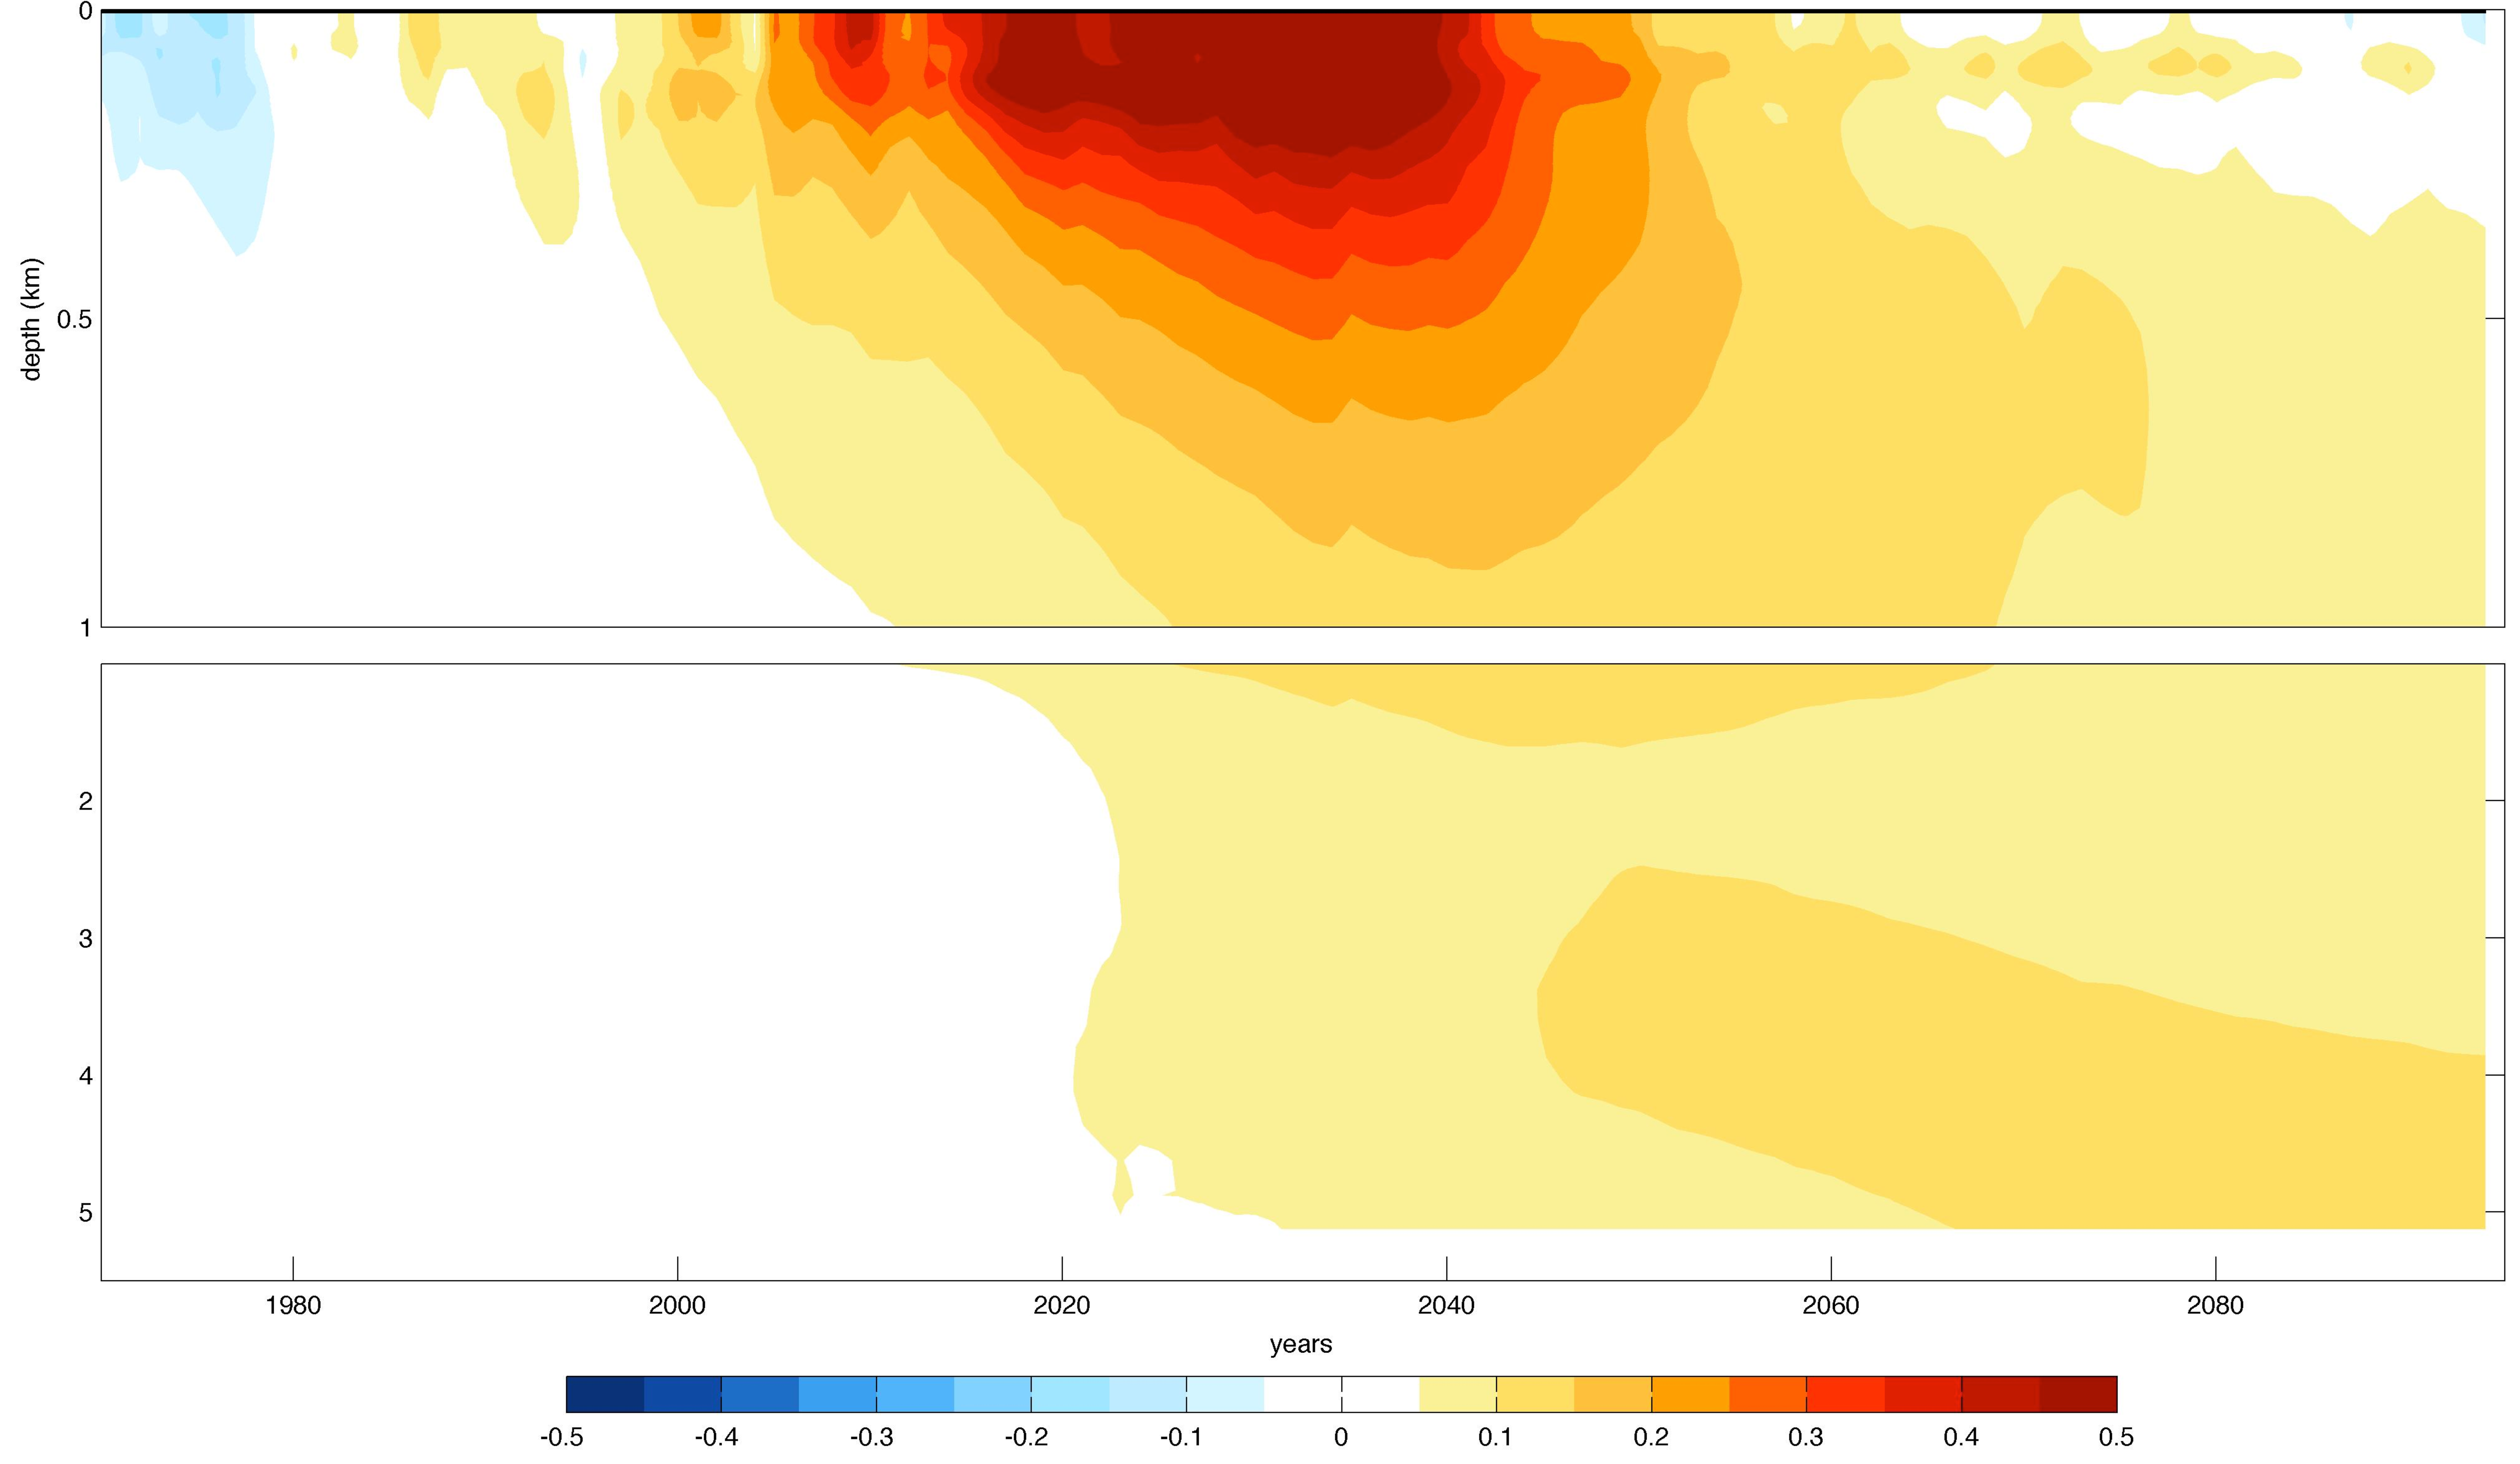
\includegraphics[width=39pc]{figures/SuppFig3.pdf}  % @@  reconfigure to horizontal layout?
\caption{\textbf{Southern Ocean temperature anomalies with time.} Annual average, Southern Ocean (averaged south of 50$^\circ$S) temperature ($^\circ$C) with depth and time as anomalies from the 1970-1999 average from 20thC. Years 1970-2004 are 20thC anomalies, 2005-2034 are RCP8.5 anomalies, and 2035 to end are Sulf anomalies.}
\label{fig:supp3}
\end{figure*}



%% Put the bibliography here, most people will use BiBTeX in
%% which case the environment below should be replaced with
%% the \bibliography{} command.

%\begin{thebibliography}{1}

%\end{thebibliography}


%\bibliographystyle{ametsoc}
\bibliography{allrefs}
% ~/bibtexrefs/allrefs  == this is version controlled now, but will have to just copy into current dir?


%% Here is the endmatter stuff: Supplementary Info, etc.
%% Use \item's to separate, default label is "Acknowledgements"



%%
%% TABLES
%%
%% If there are any tables, put them here.
%%

\end{document}
